%%%%%%%%%%%%%%%%%%%%%%%%%%%%%%%%%%%%%%%%%%%%%%%%%%%%%%%%%%%%%%%
%
% Welcome to Overleaf --- just edit your LaTeX on the left,
% and we'll compile it for you on the right. If you open the
% 'Share' menu, you can invite other users to edit at the same
% time. See www.overleaf.com/learn for more info. Enjoy!
%
%%%%%%%%%%%%%%%%%%%%%%%%%%%%%%%%%%%%%%%%%%%%%%%%%%%%%%%%%%%%%%%
\documentclass{beamer}
\usetheme{Luebeck}
\usecolortheme{seahorse}
\usepackage{graphicx}
\usepackage{amsfonts}
\usepackage{amsmath}
%Information to be included in the title page:
\title{Vapnik-Chervonenkis Dimension}
\subtitle{Mathematical Data Science Seminar}
\author{Yash Dalal}
\institute{University of Passau}
\date{10 November 2022}

\begin{document}

\frame{\titlepage}

\begin{frame}
\frametitle{Who are Vapnik and Chervonenkis}
\begin{itemize}
    \item Vladimir Vapnik and Alexey Chervonenkis are 2 Russian mathematicians.
    \item The VC dimension was developed between 1966 and 1990.
    \item Vladimir Vapnik also worked on support vector machines and structural risk minimization.
    \item There is not much information available for Alexey Chervonenkis.
    \item Vapnik-Chervonenkis dimension helps us to determine the appropriate classifier for our data.
\end{itemize}
\end{frame}

\begin{frame}
\frametitle{Definition of Vapnik-Chervonenkis Dimension}
\begin{alertblock}{Definition 1}
Let $H$ be a family of boolean functions defined on set $X$.
A subset $Y$ of $X$ is said to be shattered by $H$ if any \[g:Y\rightarrow\{0,1\}\]takes the form \[g = h_{\mid y}\] for some \[h\in H\] The VC dimension of $H$ is the largest size of a subset shattered by $H$.
\end{alertblock}
\end{frame}

\begin{frame}
\frametitle{Definition of Vapnik-Chervonenkis Dimension}
\begin{alertblock}{Definition 1}
\[\tau_H(m) = max_{|Y|=m}|h_{\mid y},h \in H|\]
\[VC(H) = sup\{m\in \mathbb{N^*} :\tau_H(m)=2^m\}\]
\end{alertblock}

\end{frame}

\begin{frame}
\frametitle{Definition of Vapnik-Chervonenkis Dimension}
\begin{alertblock}{Definition 2}
Let $H$ be a family of subsets of a set $X$. 
A subset $Y$ of $X$ is said to be shattered by $H$ if any \[Z\subseteq Y\] takes the form \[Z=Y\cap S\] for some \[S \in H\] The VC dimension of $H$ is the largest size of a subset shattered by $H$.
\end{alertblock}

\end{frame}

\begin{frame}
\frametitle{Definition of Vapnik-Chervonenkis Dimension}
\begin{alertblock}{Definition 2}
\[\tau_H(m) = max_{|Y|=m}|\{Y \cap S, S \in H\}|, Y \subseteq X\]
\[VC(H) = sup\{m\in \mathbb{N^*}:\tau_H(m)=2^m\}\]
\end{alertblock}

\end{frame}

\begin{frame}
\frametitle{Problem Solving Approach}
\item To establish that a family of subsets $H$ has VC dimension equal to d, the following points should be proved -
\begin{block}{Point 1}
There is a set $Y$ of size $d$ which is shattered by $H$. It is not necessary that all sets of size $d$ are shattered by $H$. This says that $VC(H) \geq d$.
\end{block}
\begin{block}{Point 2}
There is no set $Y$ of size $d+1$ which is shattered by $H$. This says that $VC(H) \leq d$.
\end{block}
\end{frame}

\begin{frame}
\frametitle{Example 1}
\begin{block}{Question}
Prove that for intervals the VC dimension is 2.
\end{block}
\textbf{\underline{Proof}} -\\
Let \underline{$H$ be a family of subsets} of $\mathbb{R}$ on set $X$ made of finite interval [c,e] with -\infty < c \leq e < +\infty.\\
\textbf{\underline{Point 1}} -\\
1. Consider $Y$ = \{c,e\}, such that $Y \subseteq X$.\\
2. Consider point d such that d \in (c,e).
\begin{center}
    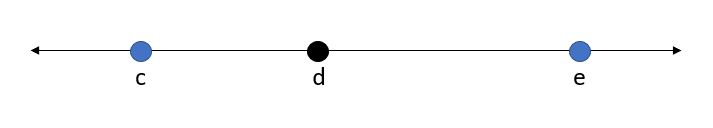
\includegraphics[scale = 0.5]{figures/Capture1.JPG}
\end{center}
\end{frame}

\begin{frame}
\frametitle{Example 1}
\textbf{\underline{Point 1}} -\\
\underline{Case 1} - \\
Let the interval be [d,d].\\
The value is 1 only on point d, on the rest of the line it is 0.
\begin{center}
    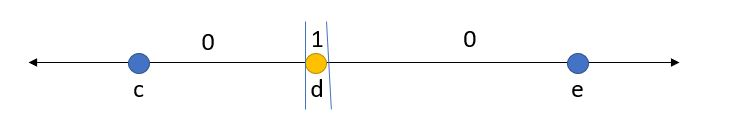
\includegraphics[scale = 0.5]{figures/Capture2.JPG}\\
    $\emptyset = \{c,e\} \cap [d,d]$
\end{center}
\end{frame}

\begin{frame}
\frametitle{Example 1}
\item \textbf{\underline{Point 1}} -\\
\underline{Case 2} - \\
Let the interval be [c,d].
\begin{center}
    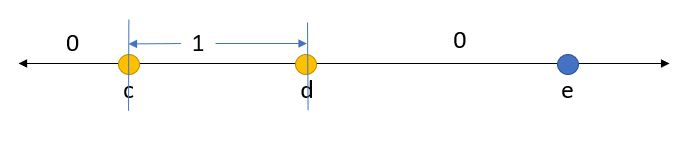
\includegraphics[scale = 0.5]{figures/Capture3.JPG}\\
    $\{c\} = \{c,e\} \cap [c,d]$
\end{center}
\end{frame}

\begin{frame}
\frametitle{Example 1}
\item \textbf{\underline{Point 1}} -\\
\underline{Case 3} - \\
Let the interval be [d,e]
\begin{center}
    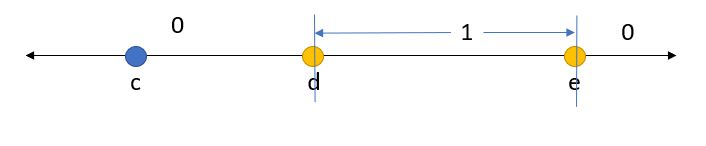
\includegraphics[scale = 0.5]{figures/Capture4.JPG}\\
    $\{e\} = \{c,e\} \cap [d,e]$
\end{center}
\end{frame}

\begin{frame}
\frametitle{Example 1}
\item \textbf{\underline{Point 1}} -\\
\underline{Case 4} - \\
Let the interval be [c,e]
\begin{center}
    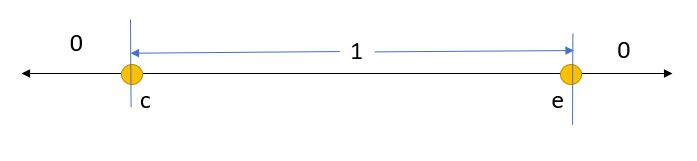
\includegraphics[scale = 0.5]{figures/Capture5.JPG}\\
    $\{c,e\} = \{c,e\} \cap [c,e]$
\end{center}
\end{frame}


\begin{frame}
\frametitle{Example 1}
\item \textbf{\underline{Point 2}} -\\
Now, let us consider set $Z $ of size 3, $\{c,d,e\}$ with $-\infty < c < d < e < \infty $.\\
\begin{center}
    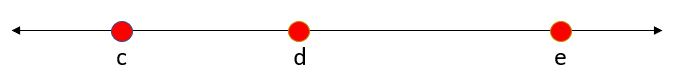
\includegraphics[scale = 0.5]{figures/Capture6.JPG}\\
\end{center}
\begin{itemize}
    \item <1-> In Point 1, $d$ was just a part of the interval (c,e), here d is a part of the set. In an interval, only 2 boundary points can be shattered.\\
    \item <2-> We know, $Y \subseteq X$ and $Z$ = \{c,e\}, where $Z \subseteq Y$.
    \item <3-> Then, set $Z \neq \{c,d,e\}$ as it cannot satisfy $Z = \{c, d, e\} \cap [c , e]$ for -\infty < c \leq e < +\infty.\\
\end{itemize}
\end{frame}

\begin{frame}
\frametitle{Example 1}
\begin{block}{Question}
Prove that for intervals the VC dimension is 2.
\end{block}
\item \textbf{From points 1 and 2 we have proved that for intervals the VC dimension is 2.}\\
\begin{center}
    Therefore, VC($H$) = $2$,\\
\end{center}
Where $H$ is a family of subsets of $\mathbb{R}$ made of finite intervals [c,e] with -\infty < c \leq e < +\infty.\\
\end{frame}


\begin{frame}
\frametitle{Example 2}
\begin{block}{Question}
Prove that for pairs of intervals the VC dimension equals 4.
\end{block}
\textbf{\underline{Proof}} -\\
Let \underline{$H$ be the family of subsets of $\mathbb{R}$ on set $X$} for the pair of intervals $[a,b] \bigcup [c,d]$ with  -\infty < a \leq b < c \leq d < +\infty.\\
Here $Y$ = \{a,b,c,d\}, where $Y \subseteq X$
\begin{center}
    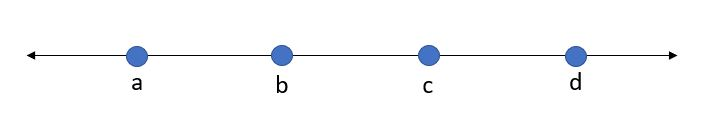
\includegraphics[scale = 0.5]{figures/Capture7.JPG}
\end{center}
\end{frame}


\begin{frame}
\frametitle{Example 2}
\textbf{\underline{Point 1}} -\\
Let us consider a set of size 4 as $Z$ = \{a,b,c,d\}.\\
If $H$ is able to shatter the set of size 4, then it can definitely shatter sets of sizes 0, 1, 2 and 3.\\
\begin{center}
    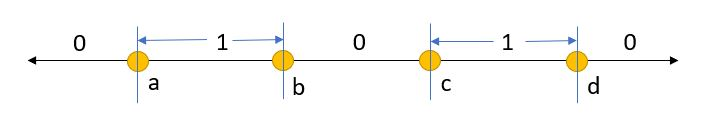
\includegraphics[scale = 0.5]{figures/Capture8.JPG}
\end{center}
\end{frame}

\begin{frame}
\frametitle{Example 2}
\textbf{\underline{Point 1}} -\\
The set $Z$ satisfies the condition $Z = \{a,b,c,d\} \cap ([a,b] \bigcup [c,d])$, where $Z \subseteq Y$\\
\begin{itemize}
    \item Hence, $H$ which is family of subsets of $\mathbb{R}$ on set $X$ can shatter set $Y$ having size 4.\\
    \item Now next let us see how it shatters subsets of sizes 0, 1, 2 and 3.
\end{itemize}
\end{frame}

\begin{frame}
\frametitle{Example 2}
\underline{Subsets of size 0 or null set} -\\
Let us consider a random point on the line where the value is 1, elsewhere the value is zero.
\begin{center}
    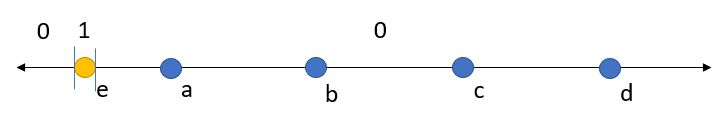
\includegraphics[scale=0.5]{figures/Capture9.JPG}
    \emptyset = $\{a,b,c,d\}\cap[e,e]$
\end{center}
\end{frame}

\begin{frame}
\frametitle{Example 2}
\underline{Subsets of size 1} -\\
\begin{center}
    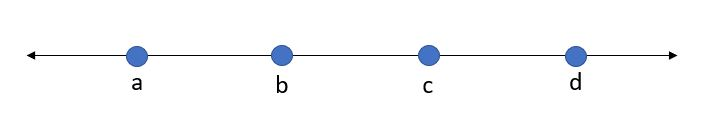
\includegraphics[scale=0.5]{figures/Capture7.JPG}
\end{center}
To shatter a single point we will use a single point on the whole line that has a value 1.
\begin{itemize}
    \item $\{a\}= \{a,b,c,d\}\cap[a,a]$
    \item $\{b\}= \{a,b,c,d\}\cap[b,b]$
    \item $\{c\}= \{a,b,c,d\}\cap[c,c]$
    \item $\{d\}= \{a,b,c,d\}\cap[d,d]$
\end{itemize}
\end{frame}

\begin{frame}
\frametitle{Example 2}
\underline{Subsets of size 2} -\\
\begin{center}
    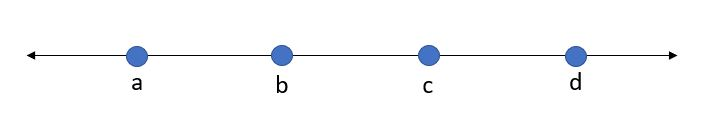
\includegraphics[scale=0.5]{figures/Capture7.JPG}
\end{center}
\begin{itemize}
    \item $\{a,b\}= \{a,b,c,d\}\cap[a,b]$
    \item $\{a,c\}= \{a,b,c,d\}\cap([a,a]\bigcup[c,c])$
    \item $\{a,d\}= \{a,b,c,d\}\cap([a,a]\bigcup[d,d])$
    \item $\{b,c\}= \{a,b,c,d\}\cap[b,c]$
    \item $\{b,d\}= \{a,b,c,d\}\cap([b,b]\bigcup[d,d])$
    \item $\{c,d\}= \{a,b,c,d\}\cap[c,d]$
\end{itemize}
\end{frame}

\begin{frame}
\frametitle{Example 2}
\underline{Subsets of size 3} -\\
\begin{center}
    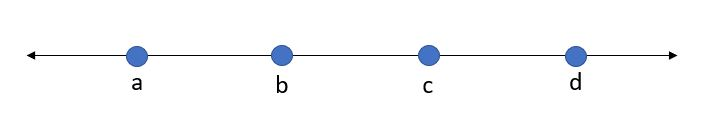
\includegraphics[scale=0.5]{figures/Capture7.JPG}
\end{center}
\begin{itemize}
    \item $\{a,b,c\}= \{a,b,c,d\}\cap([a,b]\bigcup[c,c])$
    \item $\{a,b,d\}= \{a,b,c,d\}\cap([a,b]\bigcup[d,d])$
    \item $\{a,c,d\}= \{a,b,c,d\}\cap([a,a]\bigcup[c,d])$
    \item $\{b,c,d\}= \{a,b,c,d\}\cap([b,b]\bigcup[c,d])$
\end{itemize}
\end{frame}

\begin{frame}
\frametitle{Example 2}
\underline{Subset of size 4} -\\
\begin{center}
    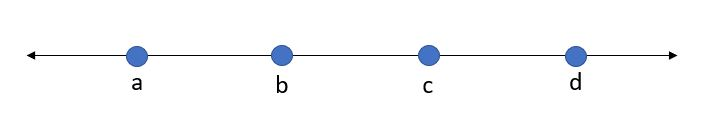
\includegraphics[scale=0.5]{figures/Capture7.JPG}
\end{center}
Lastly, the shattering of set of size 4 which we have already proven before.
\begin{itemize}
    \item $\{a,b,c,d\}= \{a,b,c,d\}\cap([a,b]\bigcup[c,d])$
\end{itemize}
\end{frame}

\begin{frame}
\frametitle{Example 2}
\textbf{\underline{Point 2}} -\\
\begin{itemize}
    \item Consider $Y$ = \{a, b, c, d, e\} having interval $-\infty < a < b < c < d < e < \infty $.
    \item We know that $Y \subseteq X$ and let $Z$ = \{a, b, c, d, e\}, $Z \subseteq Y$.
    \item Then such $Z = \{a, b, c, d, e\}$ cannot exist due to the following- 
    \begin{center}
        $Z \neq \{a, b, c, d, e\} \cap ([a,b] \bigcup [c,d])$ for -\infty < a \leq b < c \leq d < +\infty.
    \end{center}
\end{itemize}
\end{frame}

\begin{frame}
\frametitle{Example 2}
\begin{block}{Question}
Prove that for pairs of intervals the VC dimension equals 4.
\end{block}
\textbf{From points 1 and 2 we have proved that VC dimension for pairs of intervals is 4.}\\
\begin{center}
    Therefore, VC($H$) = $4$,\\
\end{center}
Where $H$ is a family of subsets of $\mathbb{R}$ on set $X$ made of finite intervals $[a,b] \bigcup [c, d]$ with -\infty < a \leq b < c \leq d < +\infty.\\
\end{frame}

\begin{frame}
\frametitle{Behavior of Shatter Function}
\begin{itemize}
    \item Shatter function grows exponentially till it reaches VC dimension.
    \item After reaching VC dimension the growth function grows polynomially.
    \item Hence, if shatter function's growth is bounded by polynomial then the VC dimension of subset is finite.
\end{itemize}
\end{frame}

\begin{frame}{Sauer Lemma}
\begin{alertblock}{Statement}
Sauer lemma conversely demonstrates that finite VC dimension implies polynomial growth.
\end{alertblock}
\begin{alertblock}{Lemma}
If $vc(H) = d$, where $H$ is family of subsets on set $X$\\ 
and $m \geq d$, where m is the maximum size of subset possible\\
then,
\[\tau_{H}(m) \leq \sum_{k=0}^{d} (_{k}^{m}) \leq \left( \frac{em}{d} \right)^{2}\]
\end{alertblock}
\end{frame}

\begin{frame}{Application of VC Dimension}
\begin{center}
    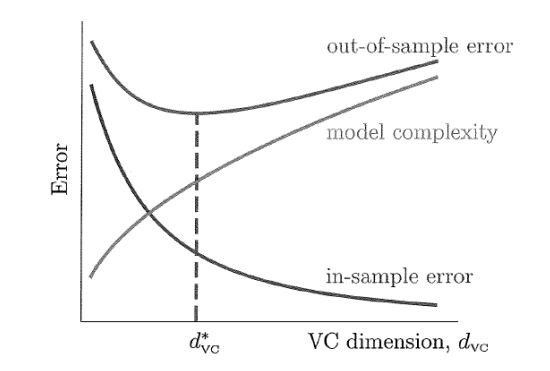
\includegraphics[scale=0.7]{figures/Capture10.JPG}\\
    \caption{\footnotesize Fig 1. Behavior of VC dimension with respect to error}
\end{center}
\end{frame}

\begin{thebibliography}{10}
\bibitem{Mathsbook} Foucart, Simon, \emph{Mathematical Pictures at a Data Science Exhibition}, Chapter 2 - Vapnik-Chervonenkis Dimension, pp. 10 - 15, Cambridge University Press, 2022.
\bibitem{wikiVapnik} Vladimir Vapnik - Wikipedia, \url{https://en.wikipedia.org/wiki/Vladimir_Vapnik}.
\bibitem{wikiChervonenkis} Alexey Chervonenkis - Wikipedia, \url{https://en.wikipedia.org/wiki/Alexey_Chervonenkis}.
\bibitem{uniLMU} Deckert, Dirk - Andre, \emph{LMU Munich, Advanced Topics in Machine Learning}, Chapter 4 - Learnability and VC Dimension, pp. 8 - 25, \url{https://www.mathematik.uni-muenchen.de/~deckert/teaching/SS17/ATML/media/VC_dimension.pdf}.
\end{thebibliography}

\begin{frame}{}
\begin{center}
    \textbf{\huge Thank You}
\end{center}
\end{frame}


\end{document}

